%%%%%%%%%%%%%%%%%%%%%%%%%%%%%%%%%%%%%%%%%%%%%%%%%%%%%%%%%%%%%%%%%%%%%%%%%%%%%%%%%%%%%%%%%%%%%%%%%%%
%%%%%%%%%%%%%%%%%%%%%%%%%%%%%%%%%%%%%%%%%%%%%%%%%%%%%%%%%%%%%%%%%%%%%%%%%%%%%%%%%%%%%%%%%%%%%%%%%%%
\chapter*{Introducci\'on}

El objetivo de este trabajo es explorar la hip\'otesis de estacionariedad en registros
polisomnogr\'aficos (EEG durante el sue\~no) en adultos mayores con Deterioro Cognitivo y de
un grupo control.

En una metodolog\'ia de estudio de casos, se describen posibles diferencias entre registros 
de sujetos en ambos grupos, lo que sugieren su utilizaci\'on como
como marcadores de uso cl\'inico en el diagn\'ostico del deterioro cognitivo en adultos mayores.

El estudio y diagnóstico de una gran cantidad de enfermedades depende de nuestra habilidad para
registrar y analizar se\~nales electrofisiol\'ogicas. 

Se suele asumir que estas se\~nales son complejas: no lineales, no estacionarias y sin equilibrio 
por naturaleza. Pero usualmente no se comprueban formalmente estas propiedades.

Correlaci\'on inter-hemisf\'erica durante el sueño MOR del Adulto Mayor con Deterioro Cognitivo.

\begin{figure}[h]
\centering
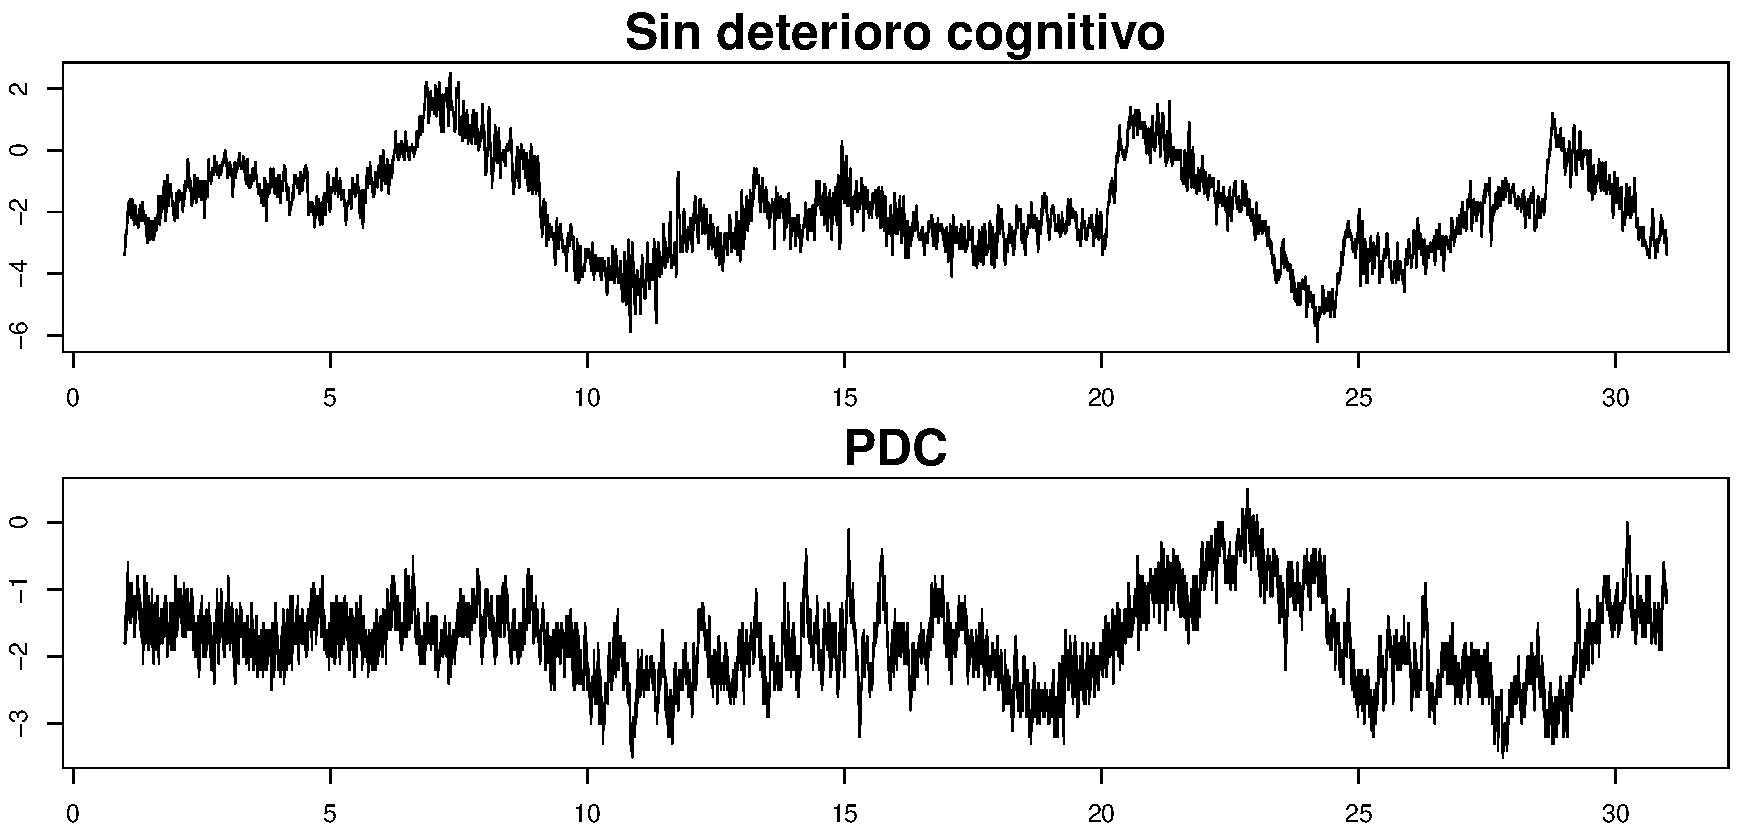
\includegraphics[width=.8\linewidth]{graficaintro.pdf}
\end{figure}

Adaptado de V\'azquez-Tagle y colaboradores (2016)

%Visualmente, el sue\~no MOR se caracteriza por movimientos oculares r\'apidos, aton\'ia muscular y 
%una actividad electroencefalogr\'afica desincronizada \cite{RosalesLagarde09}.

%%%%%%%%%%%%%%%%%%%%%%%%%%%%%%%%%%%%%%%%%%%%%%%%%%%%%%%%%%%%%%%%%%%%%%%%%%%%%%%%%%%%%%%%%%%%%%%%%%%
%%%%%%%%%%%%%%%%%%%%%%%%%%%%%%%%%%%%%%%%%%%%%%%%%%%%%%%%%%%%%%%%%%%%%%%%%%%%%%%%%%%%%%%%%%%%%%%%%%%